
%\UseRawInputEncoding
\documentclass{article}
\setcounter{secnumdepth}{0}
\usepackage[T1]{fontenc}
\usepackage[utf8]{inputenc}
%\usepackage[latin1]{inputenc}
%\usepackage[english, norsk]{babel}
\usepackage{filecontents}
\usepackage{tcolorbox}
\usepackage{url}
\usepackage{etoolbox}
\usepackage{framed}
\usepackage{framed, color}
\usepackage{xcolor}
\usepackage{mdframed}
\usepackage{float}
\usepackage{gensymb}
\usepackage{amsmath}

\definecolor{Black}{rgb}{0.0, 0.0, 0.0}

%Definer kode
\usepackage{listings}
\usepackage{color}
\definecolor{dkgreen}{rgb}{0,0.6,0}
\definecolor{gray}{rgb}{0.5,0.5,0.5}
\definecolor{mauve}{rgb}{0.58,0,0.82}

\lstset{frame=tb,
extendedchars = true,
texcl=true,
  language=C++,
  aboveskip=3mm,
  belowskip=3mm,
  showstringspaces=false,
  columns=flexible,
  basicstyle={\small\ttfamily},
  numbers=none,
  numberstyle=\tiny\color{gray},
  keywordstyle=\color{blue},
  commentstyle=\color{dkgreen},
  stringstyle=\color{mauve},
  breaklines=true,
  breakatwhitespace=true,
  tabsize=3
}

\usepackage[colorlinks]{hyperref}
\hypersetup{citecolor=Black}
\hypersetup{linkcolor=Black}
\hypersetup{urlcolor=Black}
\usepackage{cleveref}


\setlength{\parindent}{0em}
\setlength{\parskip}{1em}
%\renewcommand{\baselinestretch}{2.0}

%\renewcommand\thesubsection{\alph{subsection}}

\renewcommand{\figurename}{Figure}
\begin{document}
\author{Kent Odde}
\title{DCS3101\\Assignment 4}

\maketitle
\thispagestyle{empty}
\begin{center}
\includegraphics[width=\linewidth,height=0.2\textheight,keepaspectratio]{img/USN.png}
\end{center}
\newpage

\tableofcontents

\newpage

\section{Abstract}
This is my submission for the fourth assignment in DCS3101, Introduction to Cybersecurity, fall 2020.
%Innholdsfortegnelse
\section{Q1}
\textbf{Cybersecurity 101}
\begin{itemize}
  \item{Uses analogies to explain the history of the Internet}
  \item{Explains that the Internet was initially designed for a small number of large computers communicating}
  \item{The ease of communication on the Internet comes with a cost, and that is vulnerabilites in security}
  \item{Paints a picture of how impractical a truly secure network would be}
\end{itemize}
\textbf{Cyber Codes}
\begin{itemize}
  \item{Explains how codes are used all the time, because we communicate our messages in public}
  \item{Explains public key cryptography with analogies}
  \item{Explains what is encrypted and what is not, mentions that Email falls somewhere in between}
  \item{Explains how that almost every code ever crafted has been broken, and that the encryption mechanisms we use today, may have substantial flaws, waiting to be discovered}
\end{itemize}
\textbf{The Secret Lives of Hackers}
    \begin{itemize}
      \item{Defines hacking as creative problem solving}
      \item{Many are driven by intellectual curiosity, some do ethical hacking, whilst others have malicious intents}
      \item{They may be very competent or may use tools they don't understand}
      \item{They may have ideal goals, and feel that their goal justify their means}
    \end{itemize}
\textbf{A Cyber Privacy Parable}
\begin{itemize}
      \item{Tell why we have to be careful about what we store online}
      \item{Shows that when uploading material to social media, the content may be copied by the government or a crime ring for identity theft}
      \item{Shows how social media may sell your data to advertising agencies}
      \item{Make sure to keep software up to date, and have good passwords}
\end{itemize}
%Oppgaven
\section{Q2}

The score after playing the game through, can be seen in the figure below:
\begin{figure}[H]
 \centering
  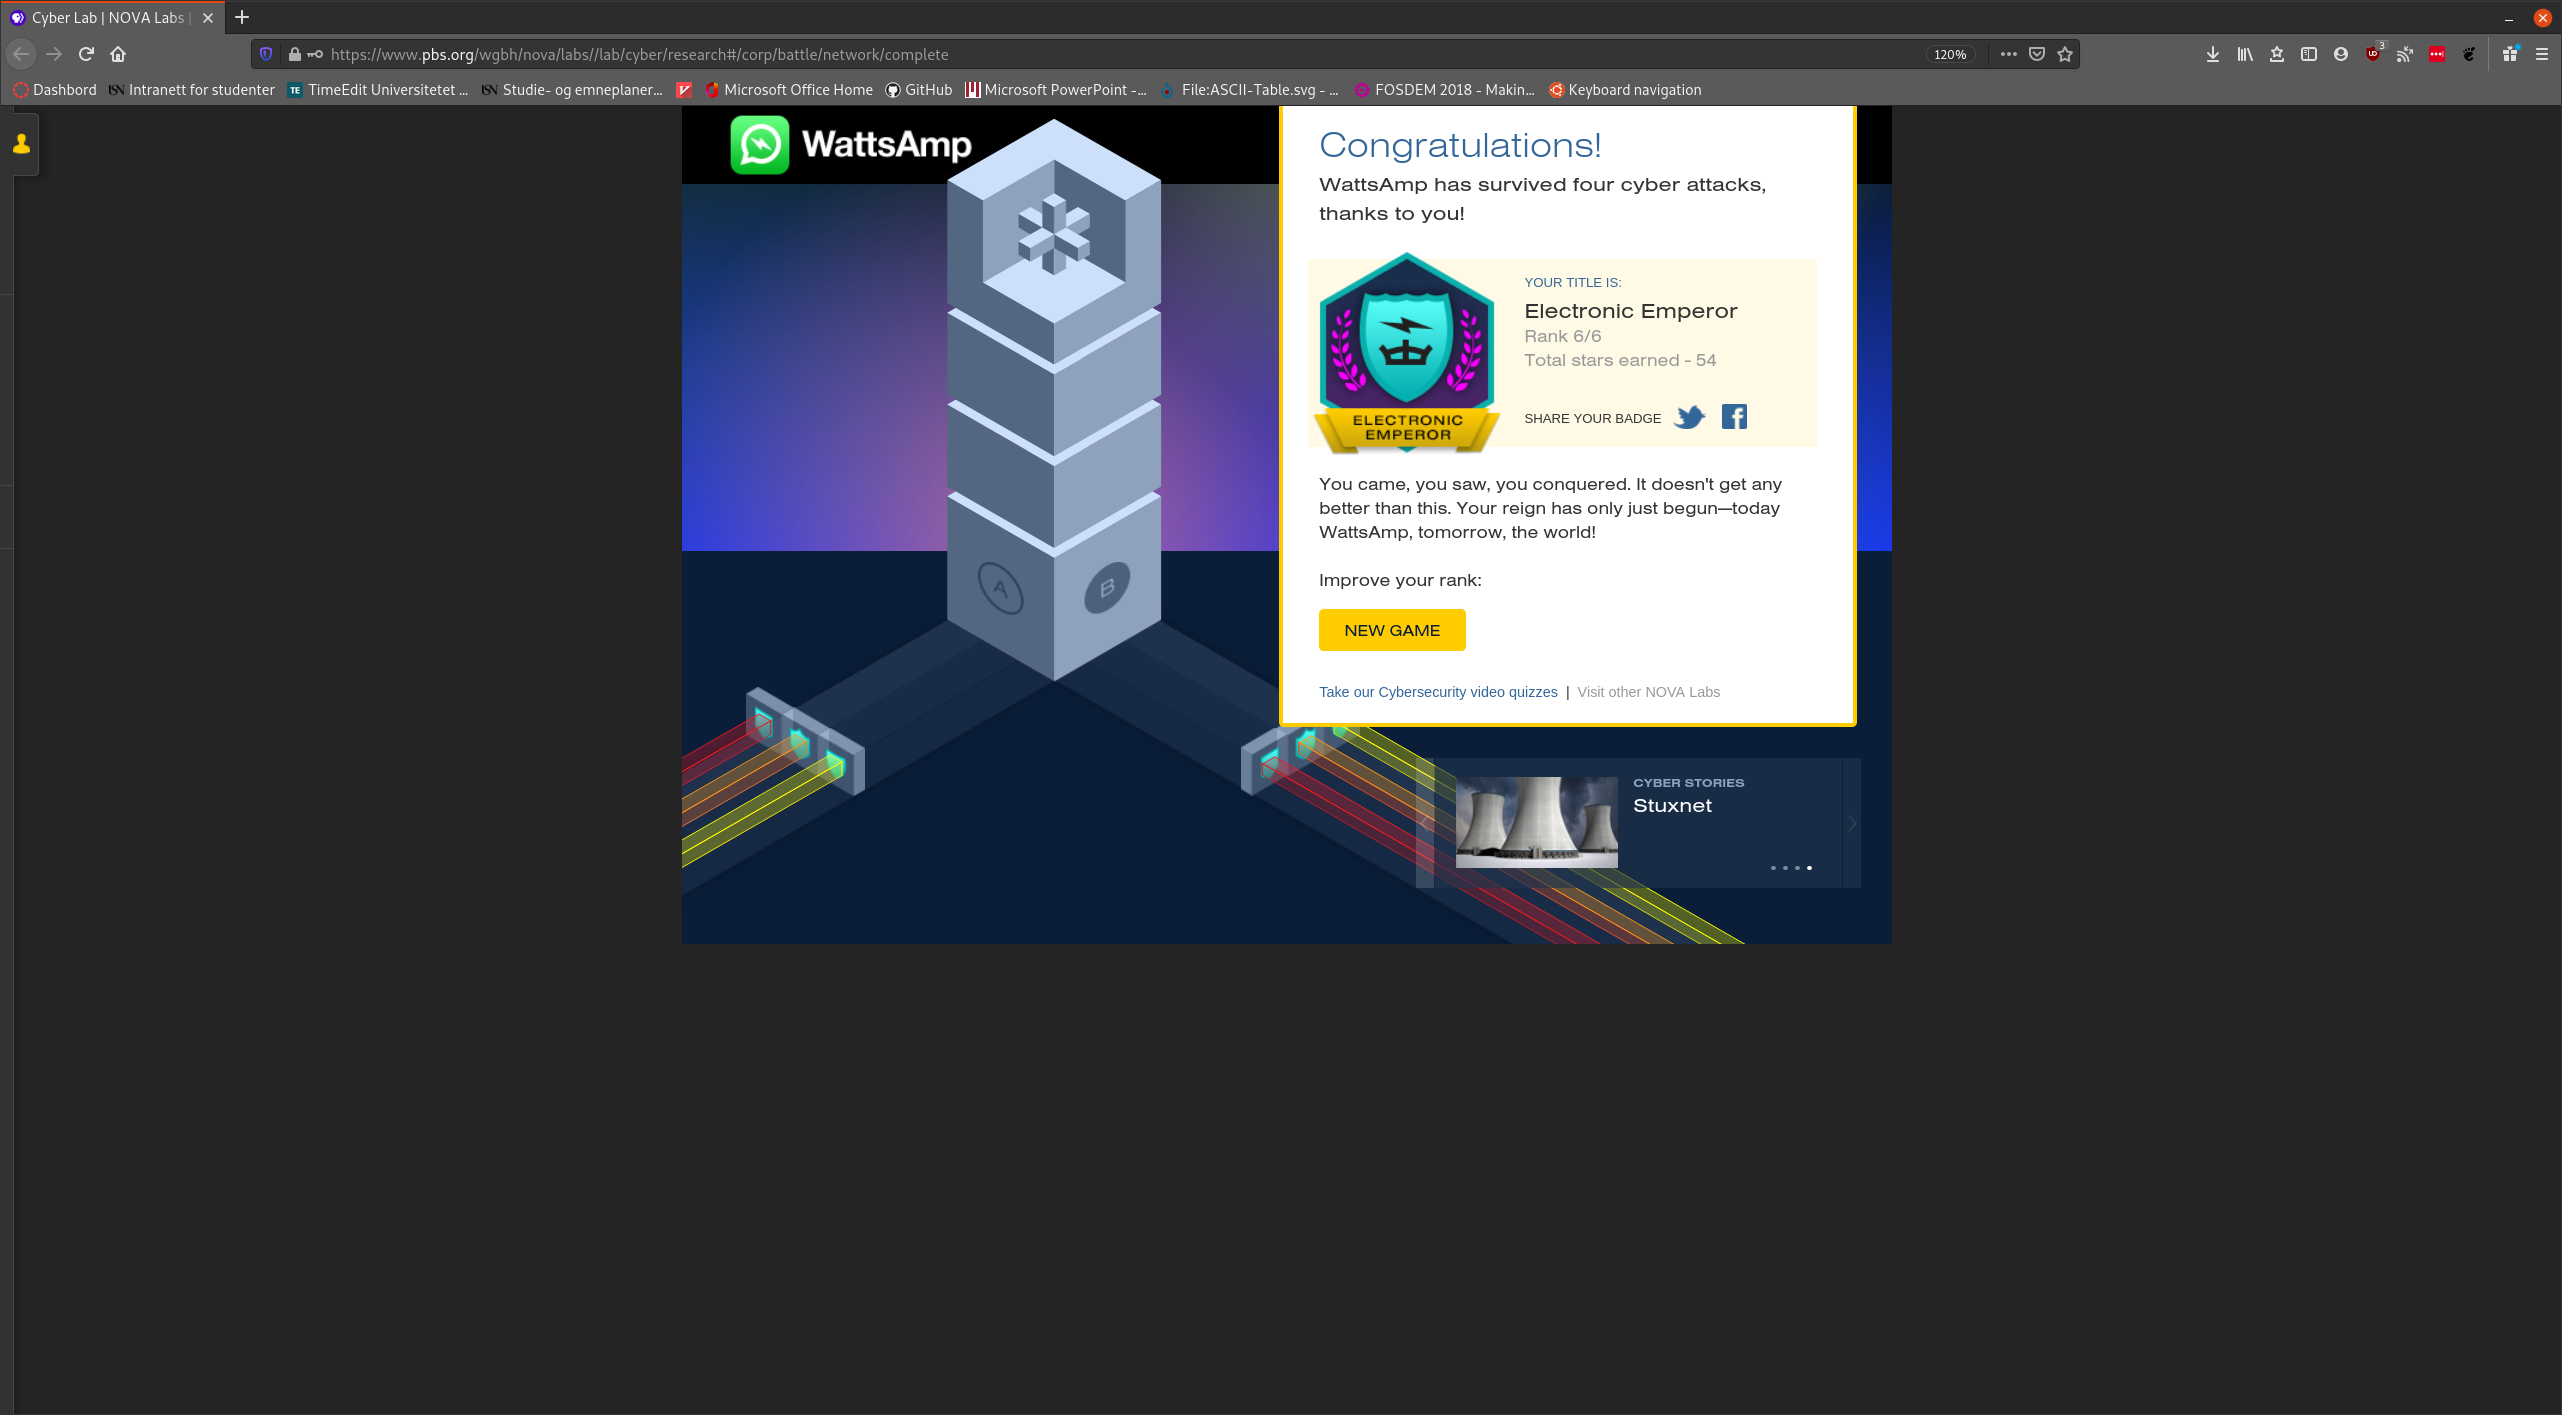
\includegraphics[width=300pt]{img/game.png}
 \caption{Score from game}
 \end{figure}

I would say that the game is well crafted, and for kids this is a great resource for learning about computer science and cyber security. However, at the university level this is too simple, and I would say that the learning outcomes are extremely limited. Having said that, I must admit that I did have fun playing it.

%Implementation
%\section{Q3}




\end{document}
